\section{$\Delta$Q adapter performance}
    We evaluated the performance of the adapter to measure its impact in a normal execution, namely we tested the following calls which represent a normal usage of the adapter.
    \begin{itemize}
        \item \texttt{start\_span} $\rightarrow$ \texttt{end\_span}.
        \item \texttt{with\_span} with the following function: \texttt{fun() $\rightarrow$ ok.}
        \item \texttt{start\_span} $\rightarrow$ \texttt{fail\_span}.
    \end{itemize}

    We ran the simulation for 25000 subsequent iterations, these are the results.
    \begin{figure}[H]
        \begin{center}
            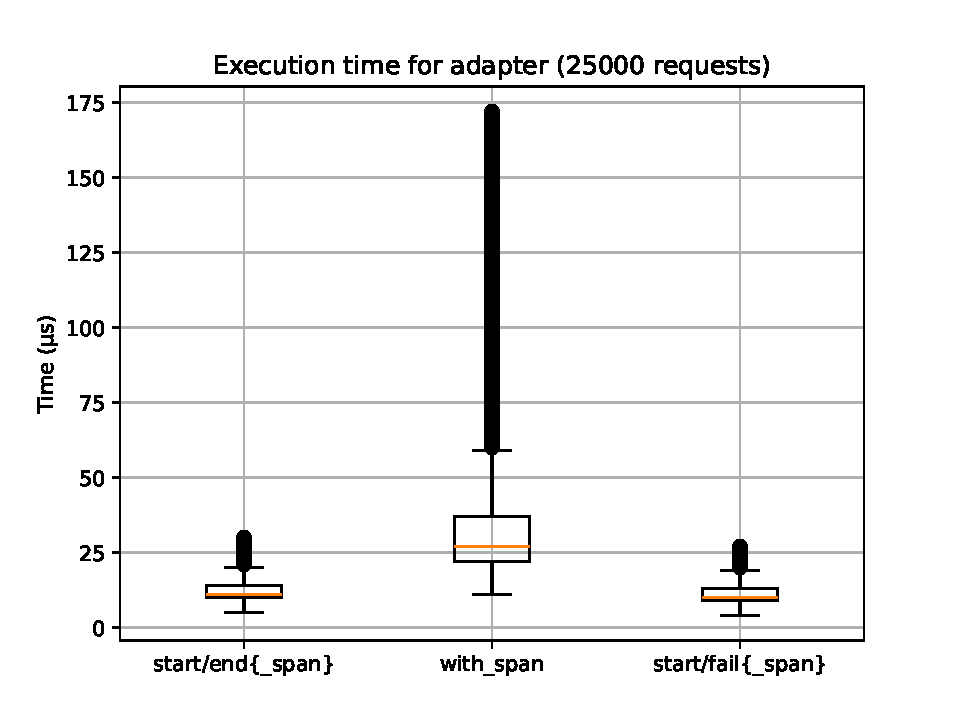
\includegraphics[width=0.8\linewidth]{img/adapter.pdf}
        \end{center}
    \end{figure}

    The overhead is minimal, around 10 microseconds on average to start and end/fail a span. The same cannot be said about with span, the increased overhead is nevertheless due to a function needing to be called inside it for it to record a span. 

